\documentclass{beamer}
\usepackage[latin1]{inputenc}

\usepackage[noend]{algpseudocode}
\usepackage[ruled]{algorithm}
\usepackage{url}
\usepackage{framed}
\usepackage{amsfonts,amsmath,amsthm}
\usepackage{graphicx}
\usepackage{url}
\usepackage{color}

\title{MCTS Based on Simple Regret}
\author{David Tolpin, Solomon Eyal Shimony}
\institute{Ben-Gurion University of the Negev\\Beer Sheva, Israel}
\date{February 22, 2012}

\AtBeginSection[]
{
  \begin{frame}<beamer>
    \frametitle{Outline}
    \tableofcontents[currentsection]
  \end{frame}
}


\begin{document}

\begin{frame}
\titlepage
\end{frame}

\begin{frame}{Hard to solve search problems}
Search problems are often hard too solve in practice when:
\begin{itemize}
\item search space is extremely large;
\item {\it and} good heuristics are unknown.
\end{itemize}
\textbf{Easier} to solve:
\begin{itemize}
\item Chess --- search space size is manageable ($10^{50}$).
\item Timetabling --- good heuristics.
\end{itemize}
\textbf{Hard} to solve:
\begin{itemize}
\item Compute Go ($10^{180}$), Poker ($10^{70}$).
\item Canadian Traveller Problem.
\end{itemize}
\end{frame}

\begin{frame}{MCTS}

{\bf M}onte {\bf C}arlo {\bf T}ree {\bf S}earch helps in large search spaces.
\begin{itemize}
\item<+-> Starts with the root only.
\item<+-> Repeats:
  \begin{enumerate}
    \item \textbf{Selection:} select a branch to explore.
    \item<+-> \textbf{Expansion:} adds children of the leaf to the stored
      tree.
    \item<+-> \textbf{Simulation:} continues search (using a simple
      strategy) until a goal state is reached.
    \item<+-> \textbf{Backpropagation:} values of each stored node 
      are updated.
  \end{enumerate}
\end{itemize}
\vspace{1em}
\textbf{Adaptive} MCTS samples `good' moves more frequently,\\
but sometimes {\bf explores} new directions.
\end{frame}

\begin{frame}{Multi-armed Bandit Problem and UCB}
Multi-armed Bandit Problem:
\begin{itemize}
\item We are given a set of $K$ arms.
\item Each arm can be pulled multiple times.
\item The reward is drawn from an {\bf unknown} (but normally {\it
    stationary} and {\it bounded}) distribution.
\item The {\bf total reward} must be maximized.
\end{itemize}

{\bf UCB} is near-optimal for MAB --- solves
{\it exploration/exploitation} tradeoff.
\begin{itemize}
\item pulls an arm that maximizes {\bf U}pper {\bf C}onfidence {\bf
    B}ound: $b_i=\overline X_i+\sqrt {\frac {c \log (n)} {n_i}}$
\item the cumulative regret is $O(\log n)$.
\end{itemize}
\end{frame}

\begin{frame}{UCT}
UCT ({\bf U}pper {\bf C}onfidence Bounds applied to {\bf T}rees) is 
based on UCB.
\begin{itemize}
\item Adaptive MCTS.
\item Applies the UCB selection scheme at each step of the rollout.
\item Demonstrated good performance in Computer Go (MoGo, CrazyStone, Fuego,
  Pachi, ...) as well as in other domains.
\end{itemize}
However, the first step of a rollout is different:
\begin{itemize}
\item The purpose of MCTS is to choose an action with the greatest utility.
\item Therefore, the {\bf simple regret} must be minimized.
\end{itemize}
\end{frame}

\begin{frame}{SRCR}

{\bf S}imple {\bf R}egret followed by {\bf C}umulative {\bf R}egret.
\begin{itemize}
\item Minimizes {\bf simple regret} at the {\bf first step}.
\item Continues with UCT from the {\bf second step on}.
\end{itemize}
\vspace{1em}
\begin{algorithmic}[1]
\Procedure{Rollout}{node, depth=1}
  \If {\Call{IsLeaf}{node, depth}}
    \State \textbf{return} 0
  \Else
    \State \textbf{if} depth=1 \textbf{then} action $\gets$ \Call{FirstAction}{node} \label{alg:srcr-first-action}   
    \State \textbf{else} action $\gets$ \Call{NextAction}{node} \label{alg:srcr-next-action}
    \State next-node $\gets$ \Call{NextState}{node, action}
    \State reward $\gets$ \Call{Reward}{node, action, next-node}
     \State \hspace{4em} + \Call{Rollout}{next-node, depth+1}
    \State \Call{UpdateStats}{node, action, reward}
  \EndIf
\EndProcedure
\end{algorithmic}
\end{frame}

\begin{frame}{Sampling for Simple Regret}
Sampling schemes for miniminizing the simple regret:
\begin{enumerate}
\item $\varepsilon$-greedy sampling.
\item a modified version of UCB (worse for cumulative, better for
  simple regret).
\item<+-> VOI-based sampling.
\end{enumerate}

\begin{itemize}
\item<+-> 1, 2 --- heuristic selection criterion, theoretical upper bounds
  can be obtained.
\item<+-> 3 --- based on principles of {\it Rational Metareasoning},
  but harder to analyze.
\end{itemize}

\end{frame}


\begin{frame}{Heuristic sampling schemes}

\onslide<+->
$\varepsilon$-greedy:
\begin{itemize} 
\item Pulls the empirically best arm with probability $\varepsilon$.
\item Any other arm with probability $\frac {1-\varepsilon} {K-1}$.
\item Exhibits exponentially decreasing simple regret.
\item Uniform sampling when $\varepsilon=\frac 1 K$, much better when
  $\varepsilon=\frac 1 2$.
\end{itemize}
\vspace{1em}
\onslide<+->
$UCB_{\sqrt{\cdot}}$ ($\sqrt{\cdot}$ instead of $\log$): 
\begin{itemize}
\item Pulls arm $i$ that maximizes
  $b_i=\overline X_i+\sqrt {\frac {c \sqrt n} {n_i}}$. 
\item Exhibits superpolynomially decreasing simple regret.
\end{itemize}
\end{frame}

\begin{frame}{VOI-aware sampling}

\begin{itemize}
\item Chooses an action with the maximum VOI estimate.
\item Estimates the VOI based on bounds on:
  \begin{itemize}
  \item the probability that one or more rollouts will make another
    action appear better than the current best;
  \item the gain that may be incurred if such a change occurs.
  \end{itemize}
\end{itemize}
\begin{eqnarray*}
VOI_\alpha&\approx&\frac {\overline X_\beta} {n_\alpha+1}
\exp\left(-2(\overline X_\alpha - \overline X_\beta)^2 n_\alpha\right)\\
VOI_i&\approx&\frac {1-\overline X_\alpha} {n_i+1}
\exp\left(-2(\overline X_\alpha - \overline X_i)^2 n_i\right),\; i\ne\alpha\nonumber\\
\mbox{where }&&\alpha=\arg\max_i \overline X_i,\quad
             \beta=\arg\max_{i,\,i\ne\alpha} \overline X_i\nonumber
\end{eqnarray*}
\end{frame}

\begin{frame}{Simple regret in MAB}

\begin{figure}[h]
  \begin{minipage}[c]{0.4\linewidth}
    \centering
    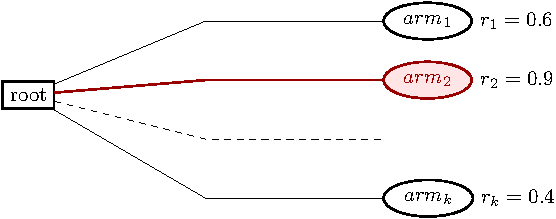
\includegraphics[scale=0.65]{onelevel-tree.pdf}\\
    {\scriptsize Fig. 1: Search tree}
  \end{minipage}
  \begin{minipage}[c]{0.4\linewidth}
    \centering
    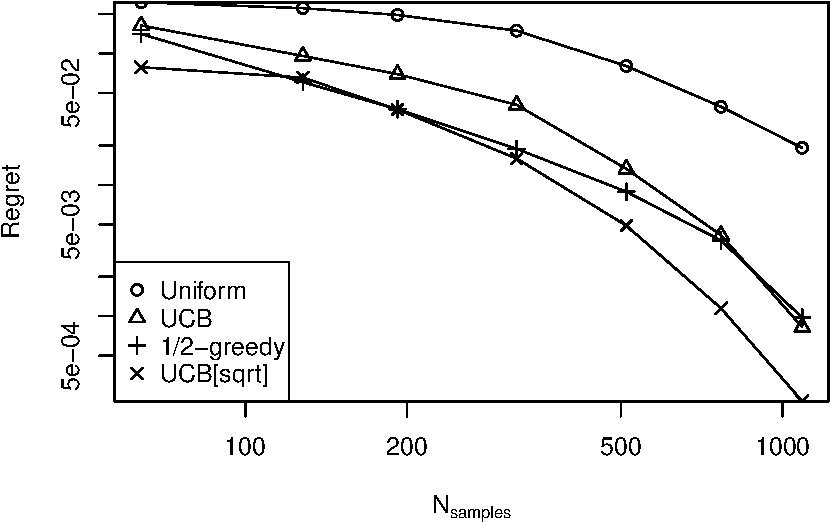
\includegraphics[scale=0.4]{flat-trilevel-k=64-uqb=8.pdf}\\
    {\scriptsize Fig. 2: Regret vs \# of samples (32 arms)}
  \end{minipage}
  \label{fig:mab-simple-regret}
\end{figure}
\begin{itemize}
\item For smaller numbers of
samples, $\frac 1 2$-greedy achieves the best
performance.
\item For larger numbers of samples, UCB$_{\sqrt{\cdot}}$
outperforms $\frac 1 2$-greedy. 
\item A combination of $\frac 1
2$-greedy  and UCB$_{\sqrt{\cdot}}$ dominates UCB over the
whole range.
\end{itemize}
\end{frame}

\begin{frame}{Monte Carlo tree search}

\begin{figure}[h]
  \begin{minipage}[c]{0.4\linewidth}
    \centering
    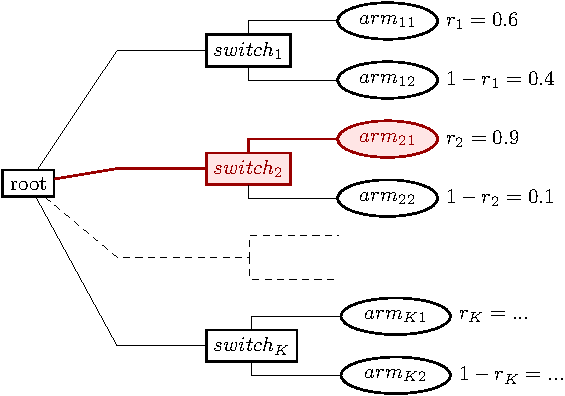
\includegraphics[scale=0.45]{twolevel-tree.pdf}\\
    {\scriptsize Fig. 1: Search tree}
  \end{minipage}
  \begin{minipage}[c]{0.4\linewidth}
    \centering
    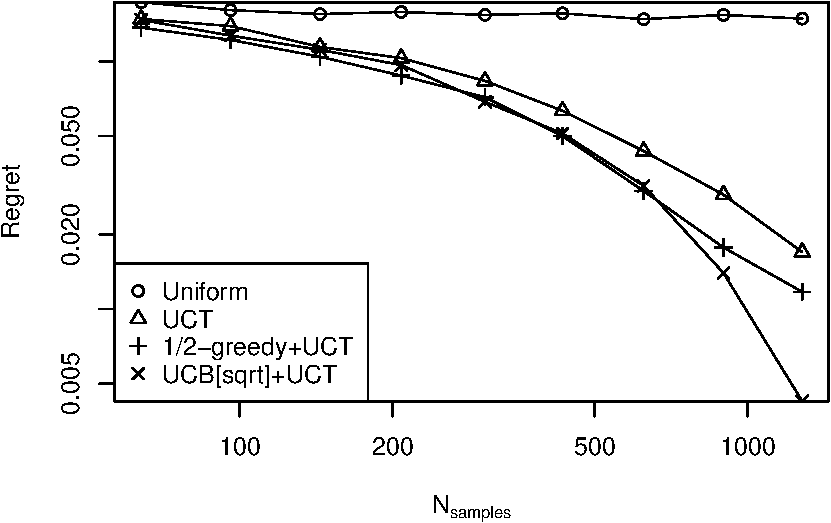
\includegraphics[scale=0.4]{tree-identity-k=16-uqb=8.pdf}\\
    {\scriptsize Fig. 2: Regret vs \# of samples (16 switches)}
  \end{minipage}
  \label{fig:mab-simple-regret}
\end{figure}
\begin{itemize}
\item Either $\frac 1
2$-greedy+UCT or UCB$_{\sqrt{\cdot}}$+UCT
gives the lowest regret.
\item UCB$_{\sqrt{\cdot}}$+UCT dominates UCT everywhere
except for small numbers of instances. 
\item The advantage of both $\frac 1
2$-greedy+UCT and UCB$_{\sqrt{\cdot}}$+UCT grows with the number of
arms.
\end{itemize}
\end{frame}

\begin{frame}{Sailing domain}
\begin{itemize}
\item A square lake.
\item A sailboat has to find the shortest path between corners.
\item The wind changes randomly.
\end{itemize}
\begin{figure}[h!]
  \begin{minipage}[b]{0.45\linewidth}
    \centering
    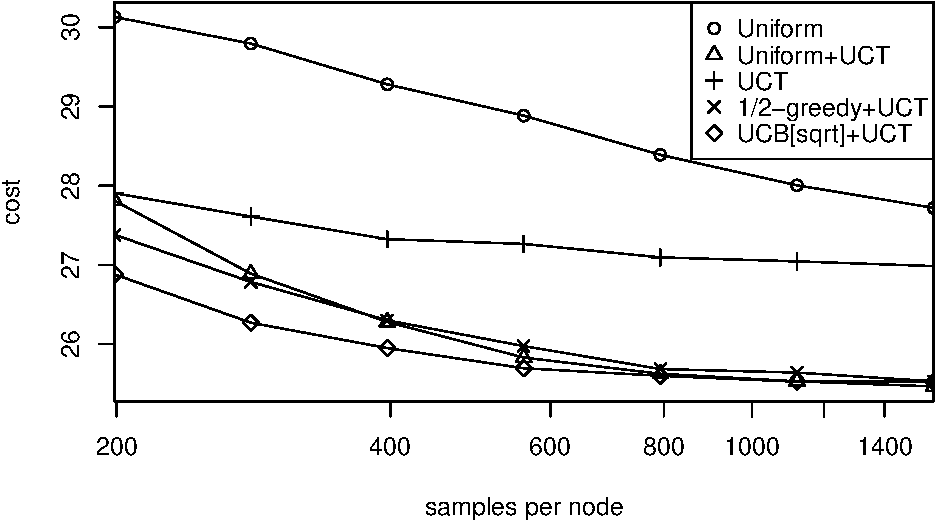
\includegraphics[scale=0.32]{costs-size=6-group=median.pdf}\\
    {\scriptsize Fig. 1: Median cost}
  \end{minipage}
  \begin{minipage}[b]{0.5\linewidth}
    \centering
    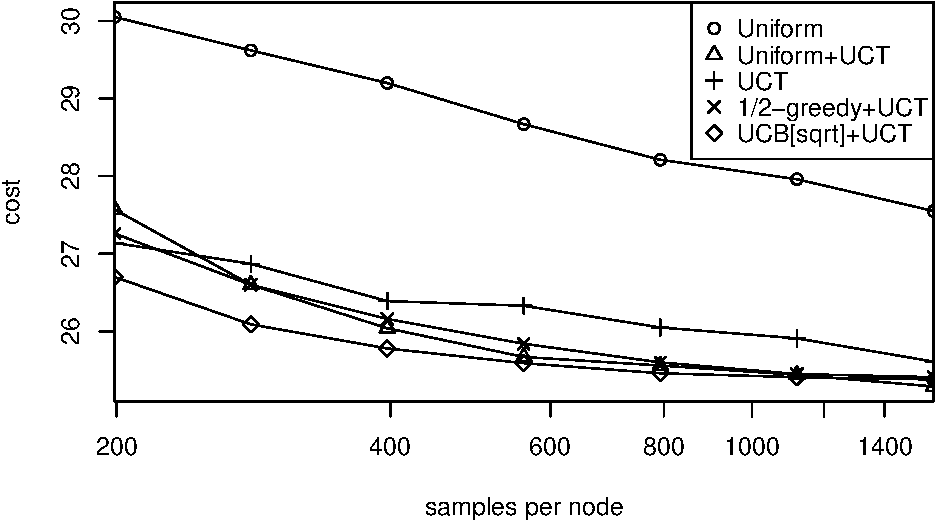
\includegraphics[scale=0.32]{costs-size=6-group=minimum.pdf}\\
    {\scriptsize Fig. 2: Minimum cost}
  \end{minipage}
  \label{fig:sailing-cost-vs-nsamples}
\end{figure}
\begin{itemize}
\item UCT is always worse than $\frac 1 2$-greedy+UCT or
UCB$_{\sqrt{\cdot}}$+UCT. 
\item UCT is sensitive to the value of $c$: the median cost is
much higher than the minimum cost.
\end{itemize}
\end{frame}

\begin{frame}{VOI-aware MCTS}
\begin{figure}[h]
  \centering
  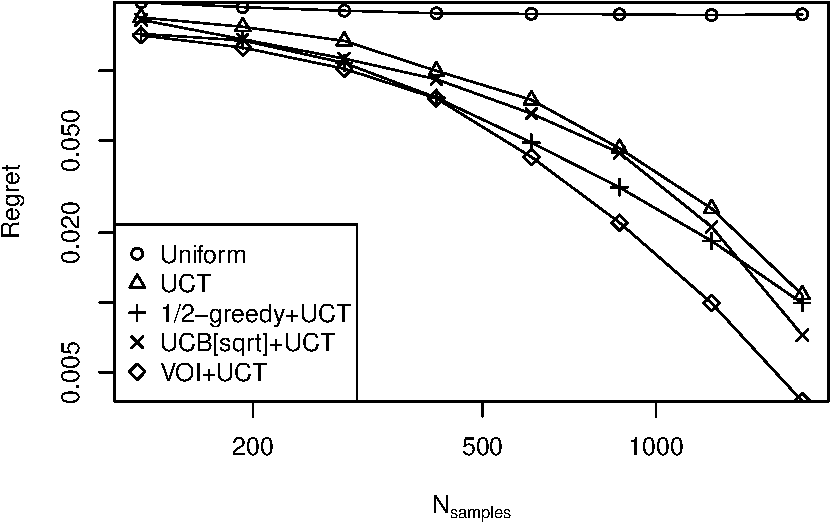
\includegraphics[scale=0.6]{tree-identity-k=32-uqb=8+voi.pdf}\\
\end{figure}
\begin{itemize}
\item The experiments were performed on
randomly generated trees.
\item VOI+UCT, the scheme based on a VOI estimate,
outperforms all other sampling schemes in this example.
\end{itemize}
\end{frame}

\begin{frame}{Summary}
\begin{itemize}
\item<+-> Improved MCTS scheme, SRCR, introduced.
\item<+-> SRCR performs better than unmodified UCT.
\item<+-> VOI-aware sampling for minimizing sampling regret proposed.
\item<+-> Better sampling schemes can be developed based on principles
  of Rational Metareasoning.
\item<+-> UCT is not well understood. Better understanding will help
  in developing efficient  MCTS schemes and adapting to different domains.
\end{itemize}
\end{frame}

\begin{frame}{}
\begin{center}
\LARGE{Thank you!}
\end{center}
\end{frame}

\end{document}
